\subsection{Rangefinder Testing}
The URG-04LX scanning laser rangefinder required an external 5V power source connection. It was connected to a lab bench power supply for all of the sensor suite's testing. Once the power supply was turned on the rangefinder's status LED illuminated, signifying that it was ready and waiting to be communicated with.

\subsubsection{Testing via the Data Viewing Tool}
The URG-04LX has a useful data viewing tool by Hokuyo Automatic Co. that was used to view, record, and replay the device's data. To use this tool, the device was connected to a computer via its USB port and the tool was launched. Figure \ref{URGBenriStandard_pic} below shows a screen capture of the application recording data captured by the rangefinder.

\begin{figure}[H]
	\centerline{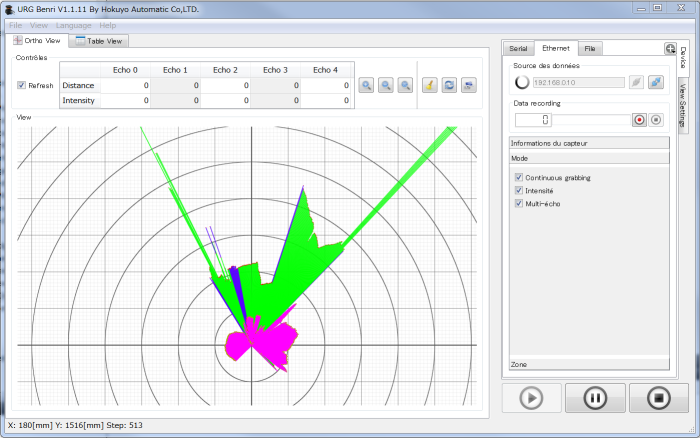
\includegraphics[width=1\textwidth]{UrgBenri_screenshot.png}}
	\caption{Screen Capture of the URG-04LX Data Viewing Tool \cite{URGBenriStandard_ref}}
	\label{URGBenriStandard_pic}
\end{figure}

Note that the start point of 0, end point of 768, and dead zone aligned to that shown in Figure \ref{rangefinder_fov}. For this project the data viewing tool was used to verify the project's 2D map output.

\subsubsection{Command Testing}
In addition to the data viewing tool, the rangefinder's commands were tested by connecting it to a laptop via its USB port. We used PuTTy, a serial console application, to communicate with the rangefinder. Figure \ref{rangefinder_putty} shows the data transfer via PuTTy between a laptop and the rangefinder. Note that PuTTy only shows data received, and that the rangefinder always echoes back the command that it receives.

\begin{figure}[H]
	\centerline{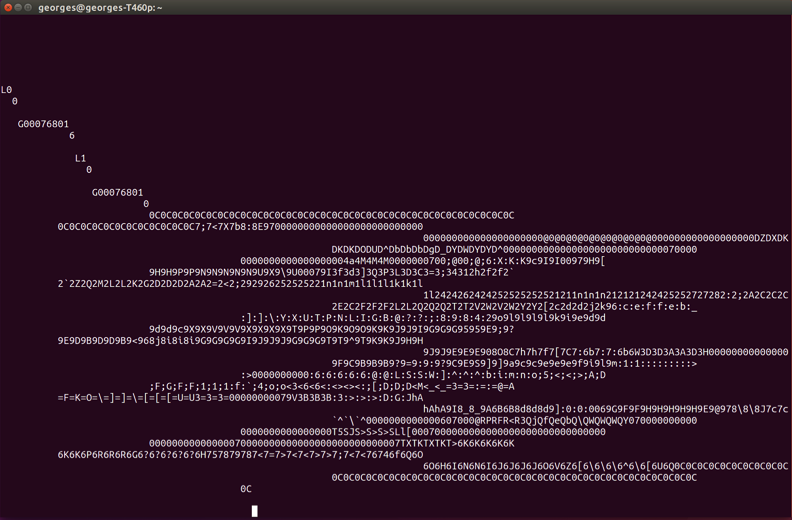
\includegraphics[width=1\textwidth]{rangefinder_putty.png}}
	\caption{Rangefinder Communication Test via PuTTy}
	\label{rangefinder_putty}
\end{figure}

The figure above shows four communication sequences used as a test. The first was the laser illumination command 'L0\textbackslash{}n'. This command turned the laser off. The rangefinder responded to this command first with the echo 'L0\textbackslash{}n', and then with '0', indicating success. The second command was the data acquisition command 'G00076801\textbackslash{}n'. The rangefinder responded with '6', indicating an error code. This specific error code was a result of the laser being off when new data was requested \cite{urg04lx_datasheet}. The third command shown was 'L1\textbackslash{}n', the laser illumination command again, which turned the laser back on. The rangefinder's response was '0' again, indicating success. The last command shown was the data acquisition command again. The rangefinder's response begins with the echo and then '0', indicating success, followed by the distance data block. The data block consisted of 768 data points, specified by the data acquisition command. By communicating with the rangefinder via PuTTy, the rangefinder's behavior was confirmed to be functional. This testing also verified that communication via the rangefinder's USB port was working.

\subsubsection{Communication via USB On-The-Go (OTG)}
With communication via the rangefinder's USB port working, this mode of communication was continued. The ZedBoard supports USB On-The-Go (OTG) which is a specification that allows USB devices to act as a host for other USB devices \cite{usb-otg}. Through USB OTG, devices choose to act as either a peripheral or a host. For the purpose of this project, the ZedBoard was expected to act as the host and initiate communication with the rangefinder. USB OTG was enabled in the Zynq7 Processing System and was controlled by the ARM Processor. The rangefinder's laser illumination command was chosen to be transmitted from the ZedBoard for this communication test. This specific command was chosen because when received, the status LED on the rangefinder blinks until the laser is turned back on. This was a simple way of verifying successful communication. In addition, when a command is transmitted via UART from the ZedBoard, its TX LED flashes. A fully successful transaction observes the ZedBoard's TX LED flashing and then the status LED on the rangefinder blinking.
\par
The ZedBoard was programmed, the rangefinder was turned on, and the two devices were connected by a standard micro-USB to mini-USB cable. The ZedBoard transmitted the command, as signified by a blink of the TX LED. However the rangefinder did not acknowledge the command; its status LED stayed lit signifying the laser stayed on. Due to this failure,\footnote{ This communication failure was most likely due to the lack of necessary hardware, as USB OTG requires an adapter that controls which device will be hosting the communication. Without this adapter, both USB devices act as a peripheral, and neither will initiate communication \cite{usb-otg}.} using USB OTG was not implemented. Instead the methodology described in Section \ref{sssec:rangefinder_communication} was implemented.

\subsubsection{Communication via Pmod}
Once we decided not to continue with USB OTG, we routed the UART signals to a Pmod connector, described in Section \ref{sssec:rangefinder_communication}. To make sure that UART via Pmod was functioning correctly, the transmit pin was measured with an oscilloscope. The laser illumination command "L0\textbackslash{}n" was transmitted and observed indicating success, as shown in the oscillogram in Figure \ref{laser_illumination}. Note that this is a TTL signal.

\begin{figure}[H]
	\centerline{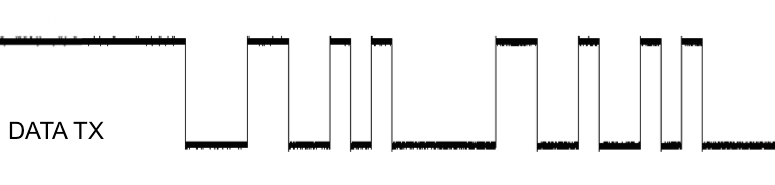
\includegraphics[width=.7\textwidth]{laser_illumination_labeled.png}}
	\caption{Laser Illumination Command TTL Oscillogram}
	\label{laser_illumination}
\end{figure}

Since the rangefinder uses RS-232 communication, an RS-232 to TTL converter with an attached breakout board was connected to the ZedBoard. The converter's V\textsubscript{CC} and GND were connected to the ZedBoard Pmod's respective V\textsubscript{CC} and GND pins. When these pins were connected, the converter's power LED turned on. In addition, the converter's RX and TX pins were connected to the ZedBoard's respective TX and RX pins. The breakout board's TX pin was measured on the oscilloscope to observe the resultant RS-232 waveform. However when the command was transmitted from the ZedBoard, there was no waveform shown on the oscilloscope. In another attempt, the converter's TX and RX pins were disconnected and swapped, so that the converter's RX and TX pins were connected to the ZedBoard's respective RX and TX pins. The laser illumination command was re-transmitted and the waveform in Figure \ref{rangefinder_rs232} was observed on the oscilloscope. The oscillogram shows a waveform from +6V to -6V, which is a valid RS-232 signal.

\begin{figure}[H]
	\centerline{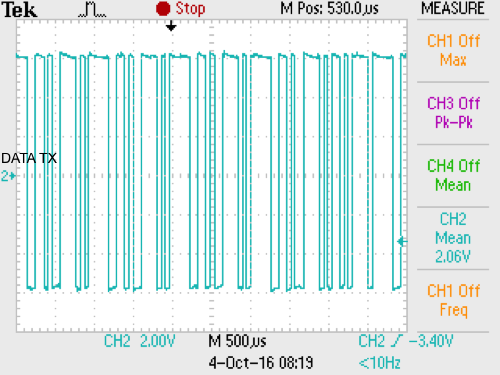
\includegraphics[width=.7\textwidth]{rangefinder_rs232_label.png}}
	\caption{Laser Illumination Command RS-232 Oscillogram}
	\label{rangefinder_rs232}
\end{figure}

With the communication functioning properly, the rangefinder's RX and TX were connected to the breakout board's respective TX and RX pins, and the laser illumination command was transmitted from the ZedBoard. The rangefinder's status LED started blinking, signifying that it received the laser illumination command and that the laser was turned off. This test's success indicated that the rangefinder's communication was completely successful.

\subsubsection{PS-PL Testing}
Once UART communication was verified, the next step was to test the PS-PL communication. In order to test the communication, UART was reconfigured in the processing system to be routed to USB UART.
\par
PL to PS communication was tested first, by using a PL button press to initiate a UART transfer. With UART communication routed to USB UART, the TX LED flashes when data is transmitted. In the PL, BTNR was used as an input and was wired into the AXI's output register, $reg\textunderscore{}data\textunderscore{}out$, in place of $slv\textunderscore{}reg0$, as seen on line 368 of the custom IP's AXI interface file located in Appendix \ref{customIPaxi}. In the PS, the data was read from the AXI bus by pointing to the address in memory where the PL's output register, $slv\textunderscore{}reg0$, is located. This address was found in the SDK in the $system.dhf$ file, which contained the hardware platform specifications. The base address was the cell with the same name as the custom IP. For this project, the base address was 43C00000\textsubscript{16}. Since $slv\textunderscore{}reg0$ was the first of the four designated memory registers, it did not need any address offset from the base address. Reading from the PL was implemented on line 30 of the PS, shown in Appendix \ref{ps_code}, by using Xilinx's built-in memory access function $Xil\textunderscore{}In32$ to read the data from the memory address that is $baseaddr\textunderscore{}p.$\footnote{ This could also have been accomplished by using a pointer to read the data from the memory address that is $baseaddr\textunderscore{}p$.} Once the setup was complete, the ZedBoard was programmed and connected to a serial console. BTNR was pressed and the TX LED lit up, indicating that PL to PS communication was functioning properly.
\par
PS to PL communication was tested next per use of the VGA screen. For this test, the PS was intended to receive the transmit signal from the PL and then wait for 768 data points to be received, just as if the rangefinder were connected. Since UART was routed to USB UART, the ZedBoard communicated with a serial console instead of the rangefinder. Through the serial console, rangefinder communication was simulated by inputting a test block of rangefinder data. The data was written to the PL one data point at a time by writing to $slv\textunderscore{}reg1$, as shown on line 239 of the custom IP's AXI interface file located in Appendix \ref{customIPaxi}. This register is located one memory register from the base address of the custom IP because it is the second of the four designated memory registers. The function $Xil\textunderscore{}Out32$ was first tested but no results were observed, so a pointer was used to write to the base address offset by one memory register. This is seen on line 198 of the PS, in Appendix \ref{ps_code}. The data written to $slv\textunderscore{}reg1$ was the distance data point combined with a data valid flag and the rangefinder step. These were manipulated to fit into one 32-bit integer by shifting each to a unique bit location of a buffer, $data\textunderscore{}enable\textunderscore{}step$.
\par
To test data accuracy in addition to PS to PL communication, the test block of rangefinder data sent from the serial console was constant. With data constant across all steps of the rangefinder's field of view, the intended result was $270^\circ$ of a circle drawn around the rangefinder on the VGA screen. With the VGA module set up and the rangefinder data processing ready to be tested, the ZedBoard was programmed. When BTNR was pushed, an image similar to Figure \ref{badCircle} was observed on the VGA screen with the red dot being the device and the black lines being the rangefinder's distance data.

\begin{figure}[H]
	\centerline{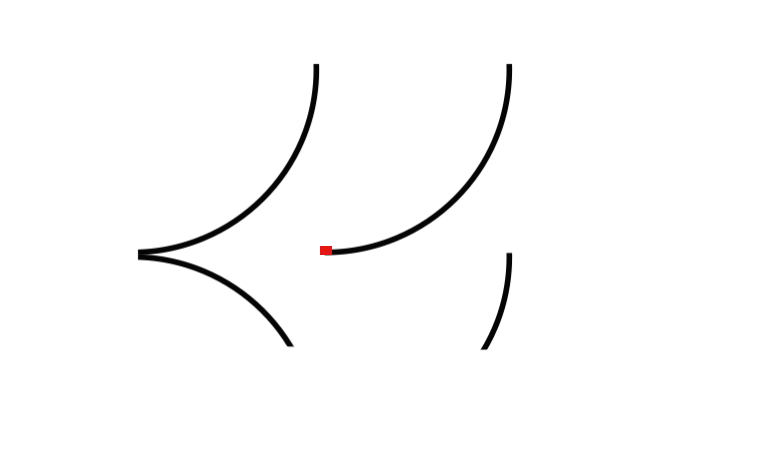
\includegraphics[width=.5\textwidth]{badCircle.png}}
	\caption{PS to PL Communication Test with Constant Data}
	\label{badCircle}
\end{figure}

Although a circle was not observed, this test confirmed the PS to PL communication was functioning properly. The shape appeared to be four quadrants of a circle, except in the wrong orientation. Since the lines seem semi-circular, the polar-to-rectangular transformation was deemed successful. The problem was a minor sign issue with the rangefinder's data processing in the PL. The signs in each necessary quadrant were fixed and the test was repeated, resulting in Figure \ref{goodCircle} being observed on the VGA screen.

\begin{figure}[H]
	\centerline{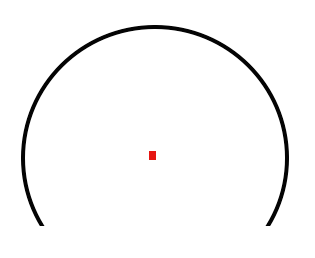
\includegraphics[width=.4\textwidth]{goodCircle.png}}
	\caption{PS to PL Communication with Constant Data and Revised Data Processing}
	\label{goodCircle}
\end{figure}

With the PS-PL communication and rangefinder data processing functioning perfectly, the rangefinder itself was attached and tested.

\subsubsection{Data Testing}
UART was re-routed to the PS Pmod in order to test the entire rangefinder implementation. The rangefinder was powered by the lab bench power supply and was connected on the RS-232 breakout side of the RS-232 to TTL converter, with the ZedBoard connected to the TTL side. The ZedBoard was connected to the VGA screen, and then was programmed. BTNR was pushed to initiate the UART transfer and Figure \ref{first} shows the VGA output. This VGA output shows the rangefinder with a wall directly in front of it.

\begin{figure}[H]
	\centerline{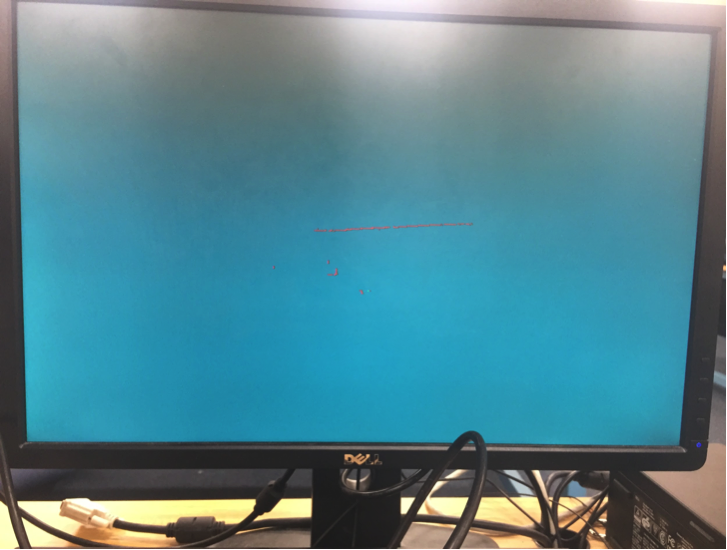
\includegraphics[width=.7\textwidth]{first.png}}
	\caption{Rangefinder Data Observed on VGA Screen}
	\label{first}
\end{figure}

Next BTNR was pushed again to start another data transfer, but there was no observed functionality. The button was held down until the subsequent data transfers in Figure \ref{subsequent} were observed on the VGA screen.

\begin{figure}[H]
	\centerline{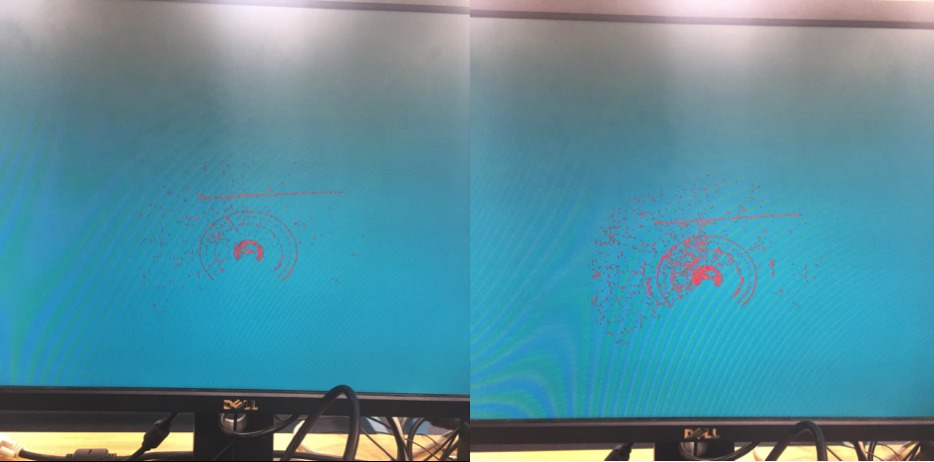
\includegraphics[width=.9\textwidth]{subsequent.jpg}}
	\caption{Subsequent Rangefinder Data Observed on VGA Screen}
	\label{subsequent}
\end{figure}

In the SDK the PS was not accounting for enough data points. By design, when the rangefinder receives a command from the ZedBoard it echoes back the command. The PS used this as a test to ensure data accuracy. When not enough data was being accounted for, the extra data was writing into the next data transfer's input echo buffer. As a result, the echo received from the rangefinder did not match the command transmitted and the rest of the data was garbage. The PS was edited to account for all of the data points and the rangefinder was tested again. Figure \ref{labtest1} shows the initial data transfer of this test, and the 2D florplan was compared to the objects around it.

%\begin{figure}[H] 
%	\begin{subfigure}{1\textwidth}
%	\centering
%		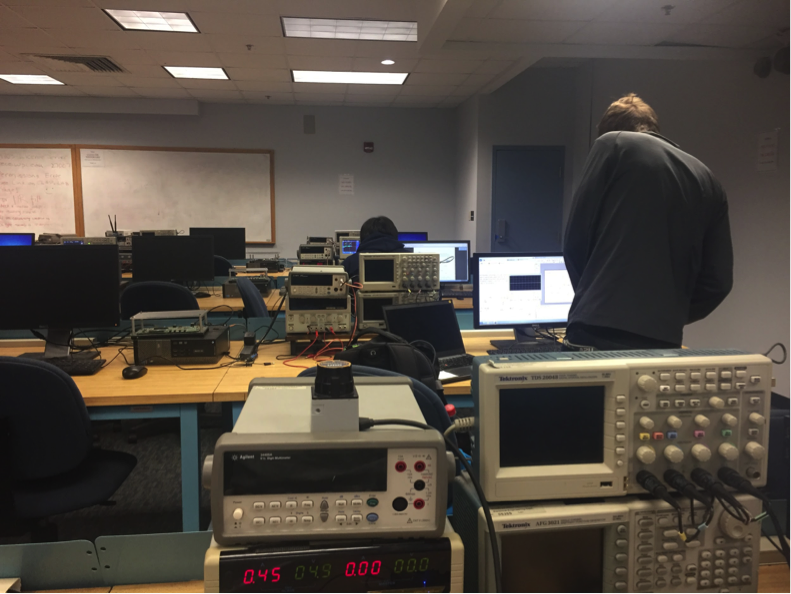
\includegraphics[width=0.8\linewidth]{labtest1_1.png}
%		\caption{Lab at WPI with $180^\circ$ Change of Orientation}
%		\label{lab1}
%	\end{subfigure}
%	\begin{subfigure}{1\textwidth}
%	\centering
%		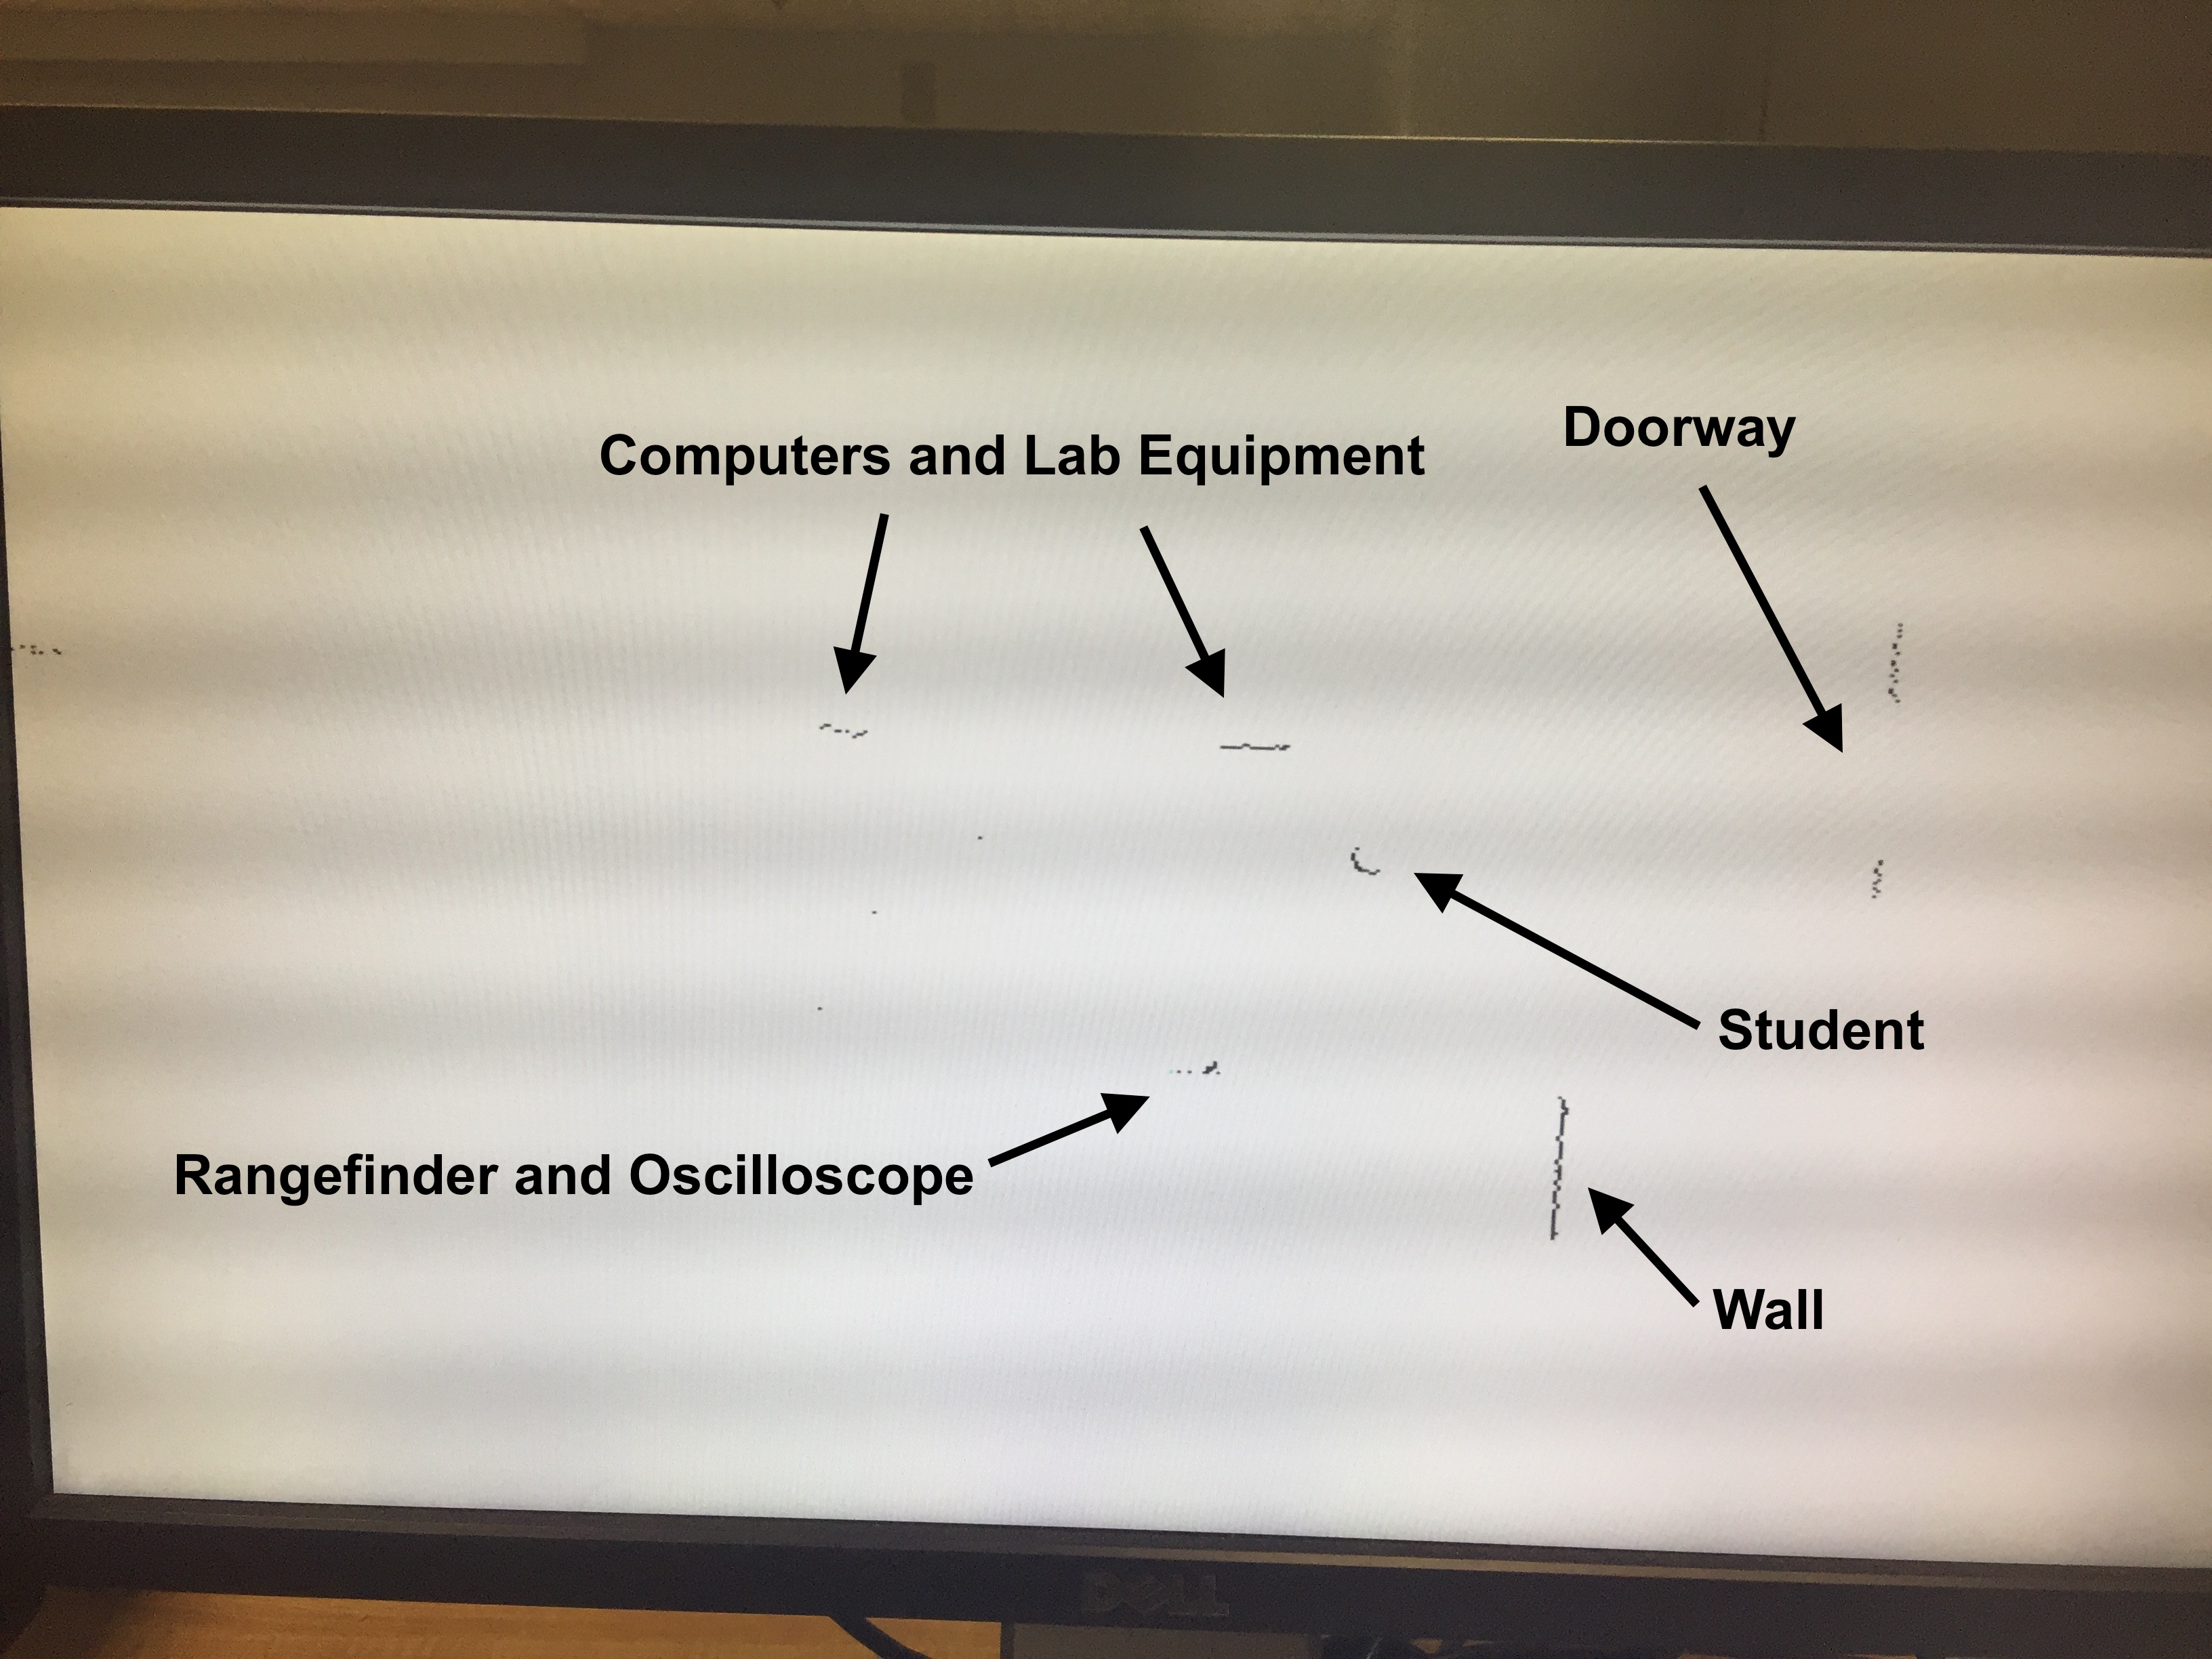
\includegraphics[width=0.8\linewidth]{lab_front.JPG}
%		\caption{2D Rangefinder "Floorplan" of Lab at WPI}
%		\label{floorplan1}
%	\end{subfigure}
%	\caption{First Lab Test of Rangefinder Functionality}
%	\label{labtest1}
%\end{figure}

%In Figure \ref{labtest1}(\subref{floorplan1}), the data points called out in the 2D floorplan include a wall directly to the right of the device, a doorway, a student, computers, lab equipment, and the rangefinder. Note that only the objects that are coplanar with the rangefinder's laser are detected by it, and are the only objects shown on the 2D floorplan. This test verified that the 
%\par
%Next, the screen was cleared, the rangefinder was rotated $180^\circ$, and the process was repeated.

\begin{figure}[H] 
	\begin{subfigure}{1\textwidth}
	\centering
		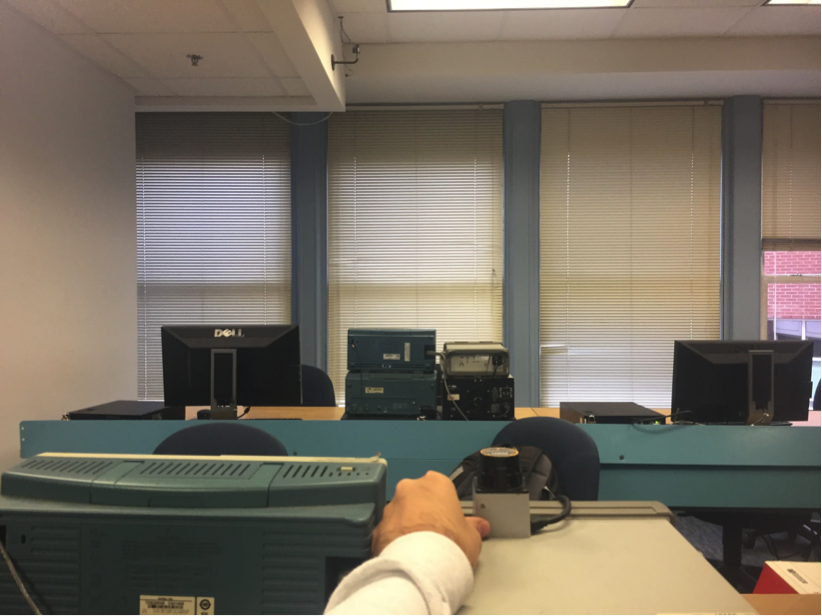
\includegraphics[width=0.8\linewidth]{labtest2_1.png}
		\caption{Lab at WPI}
		\label{lab2}
	\end{subfigure}
	\par
	\begin{subfigure}{1\textwidth}
	\centering
		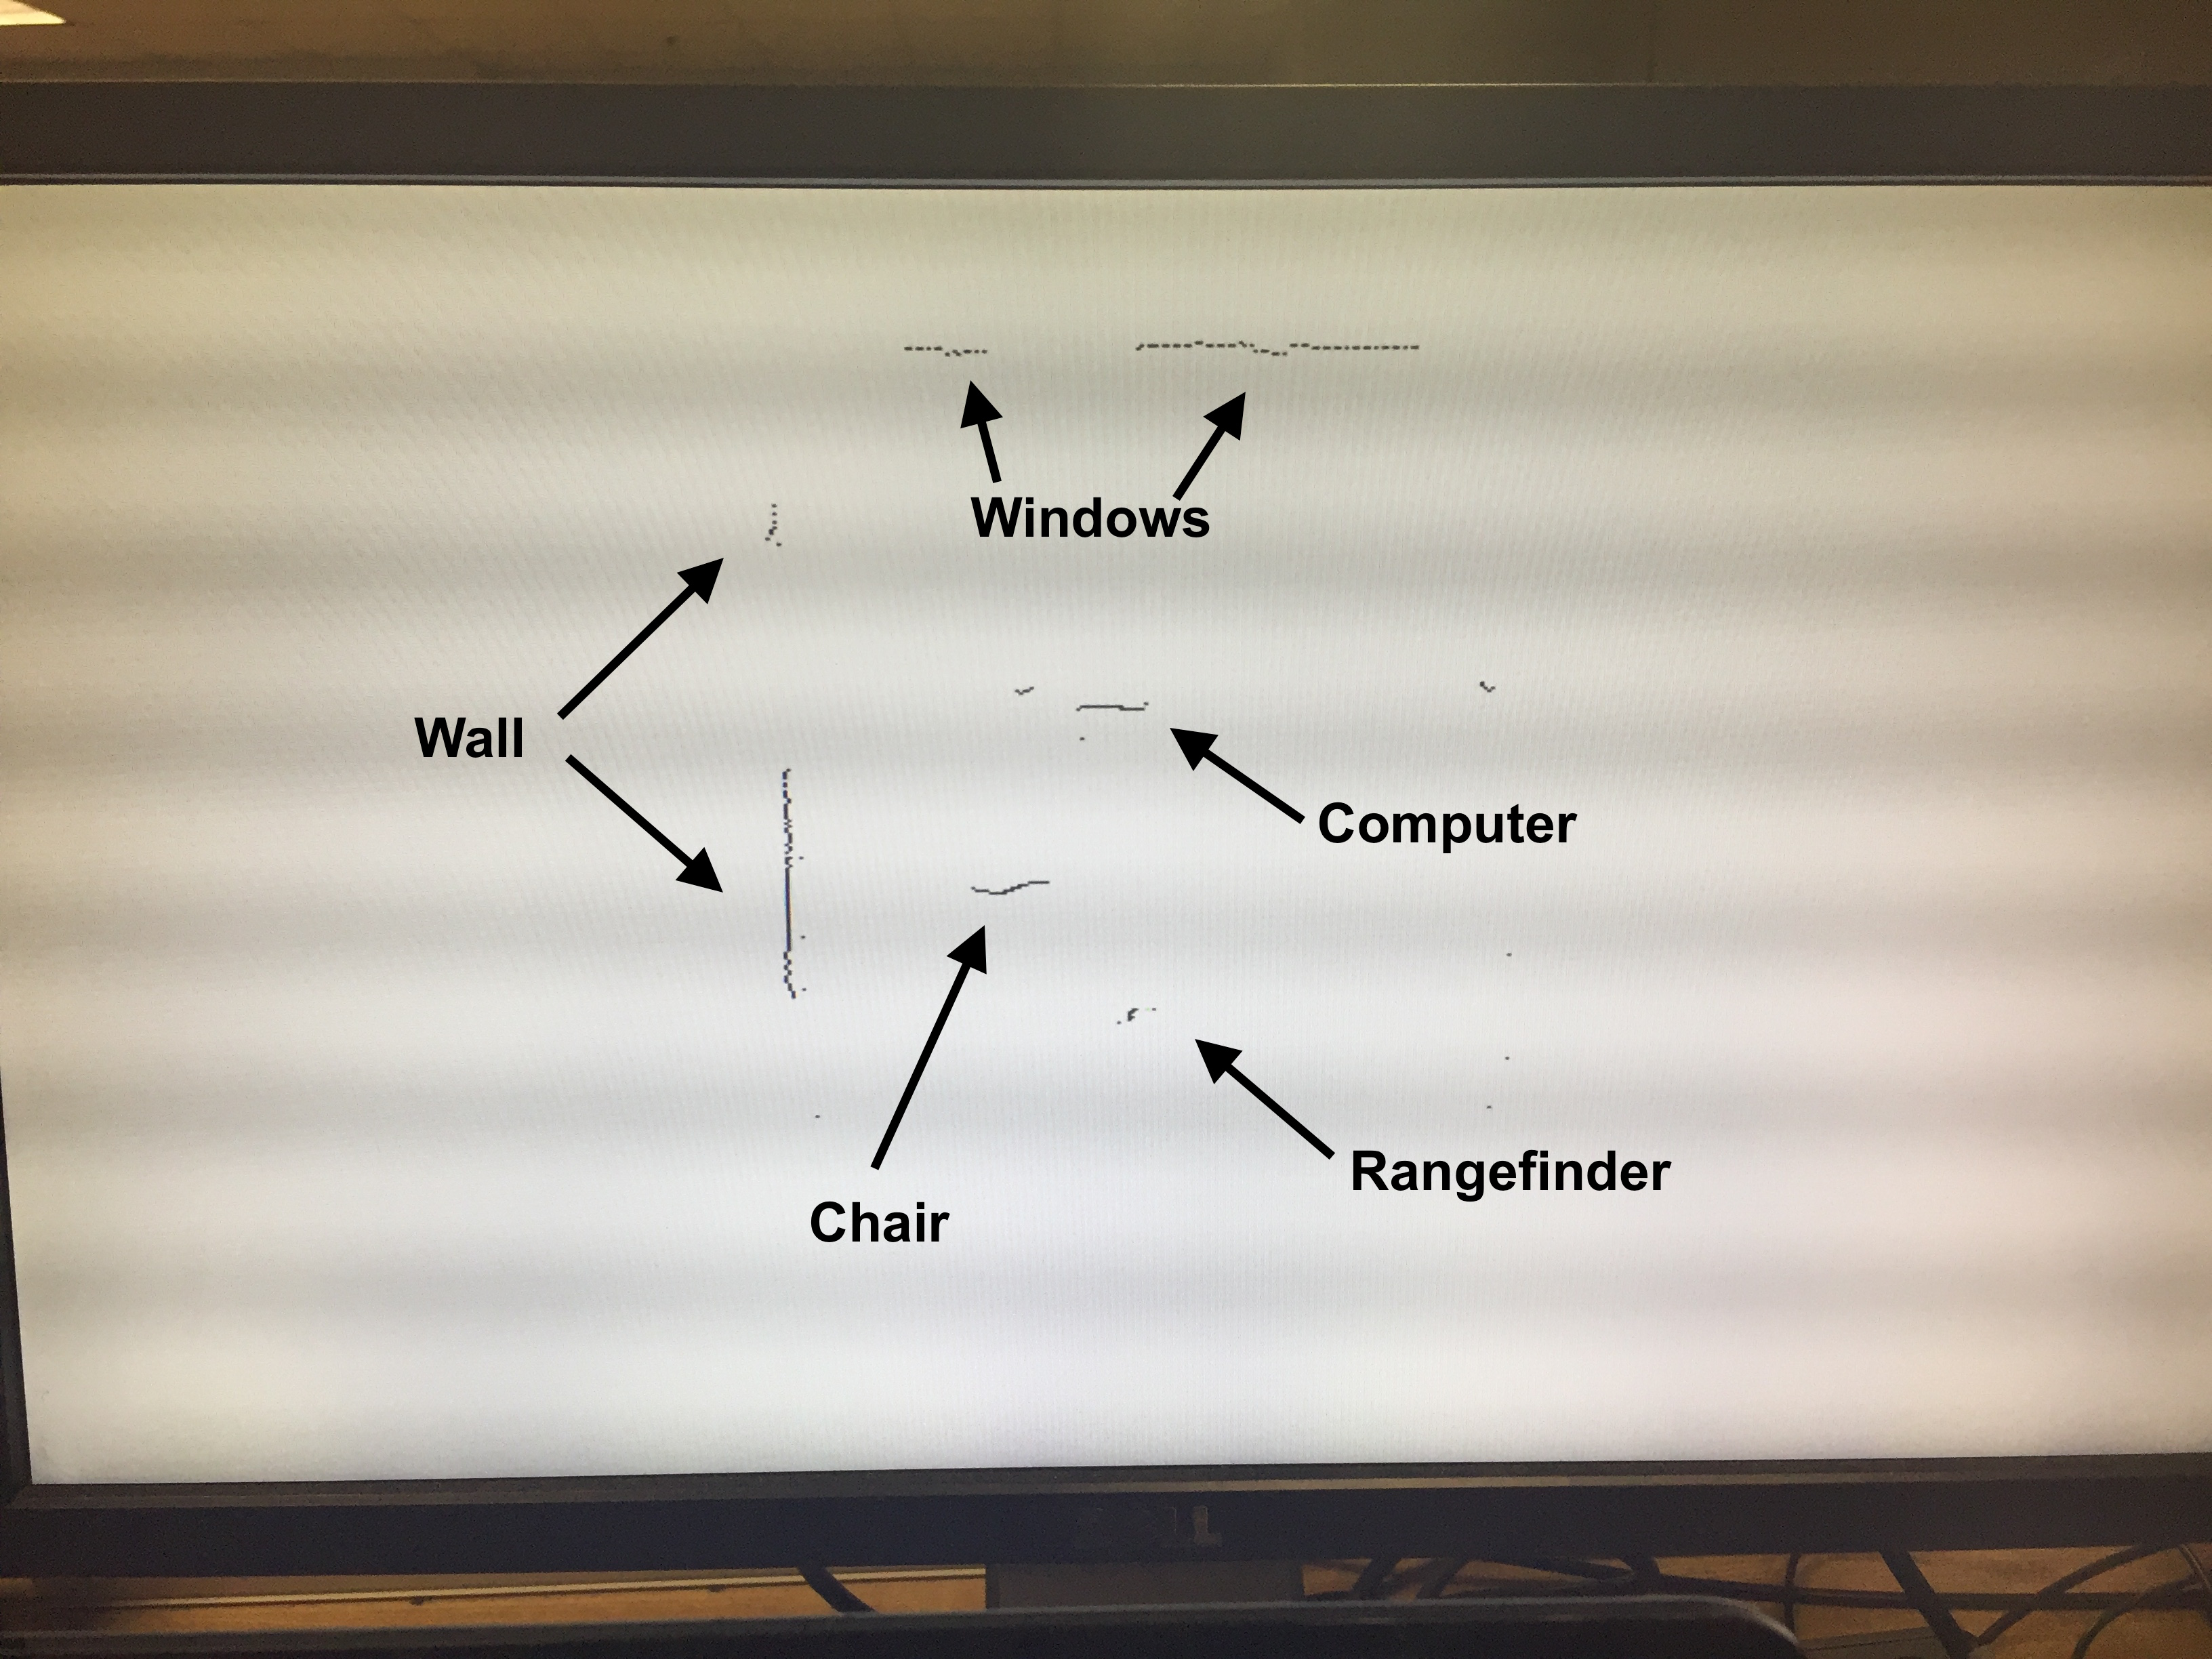
\includegraphics[width=0.8\linewidth]{lab_back.JPG}
		\caption{2D Rangefinder "Floorplan" of Lab at WPI}
		\label{floorplan1}
	\end{subfigure}
	\caption{2D Floorplan of Lab}
	\label{labtest1}
\end{figure}

In Figure \ref{labtest1}\subref{floorplan1} the data points called out in the 2D floorplan include a wall directly to the left of the device, a chair, computers, windows, and the rangefinder. These objects' locations on the floorplan corresponded to their actual locations, so the rangefinder's accuracy was confirmed.
\par
Next, the rangefinder was rotated $180^\circ$ and the button was pushed again to test the rangefinder's subsequent triggering functionality. Figure \ref{labtest2} shows the rangefinder's view when it was rotated $180^\circ$, and the resultant VGA output.

\begin{figure}[H] 
	\begin{subfigure}{1\textwidth}
	\centering
		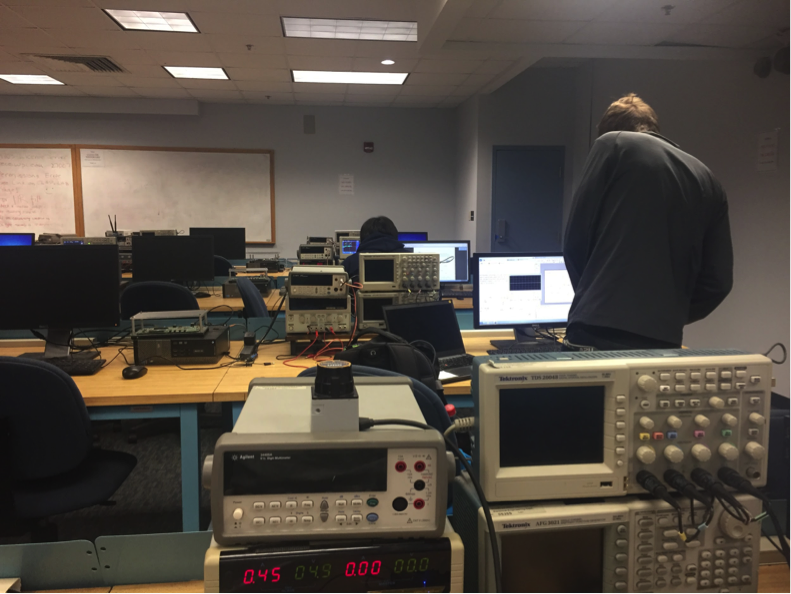
\includegraphics[width=0.8\linewidth]{labtest1_1.png}
		\caption{Lab at WPI with $180^\circ$ Change of Orientation}
		\label{lab1}
	\end{subfigure}
	\begin{subfigure}{1\textwidth}
	\centering
		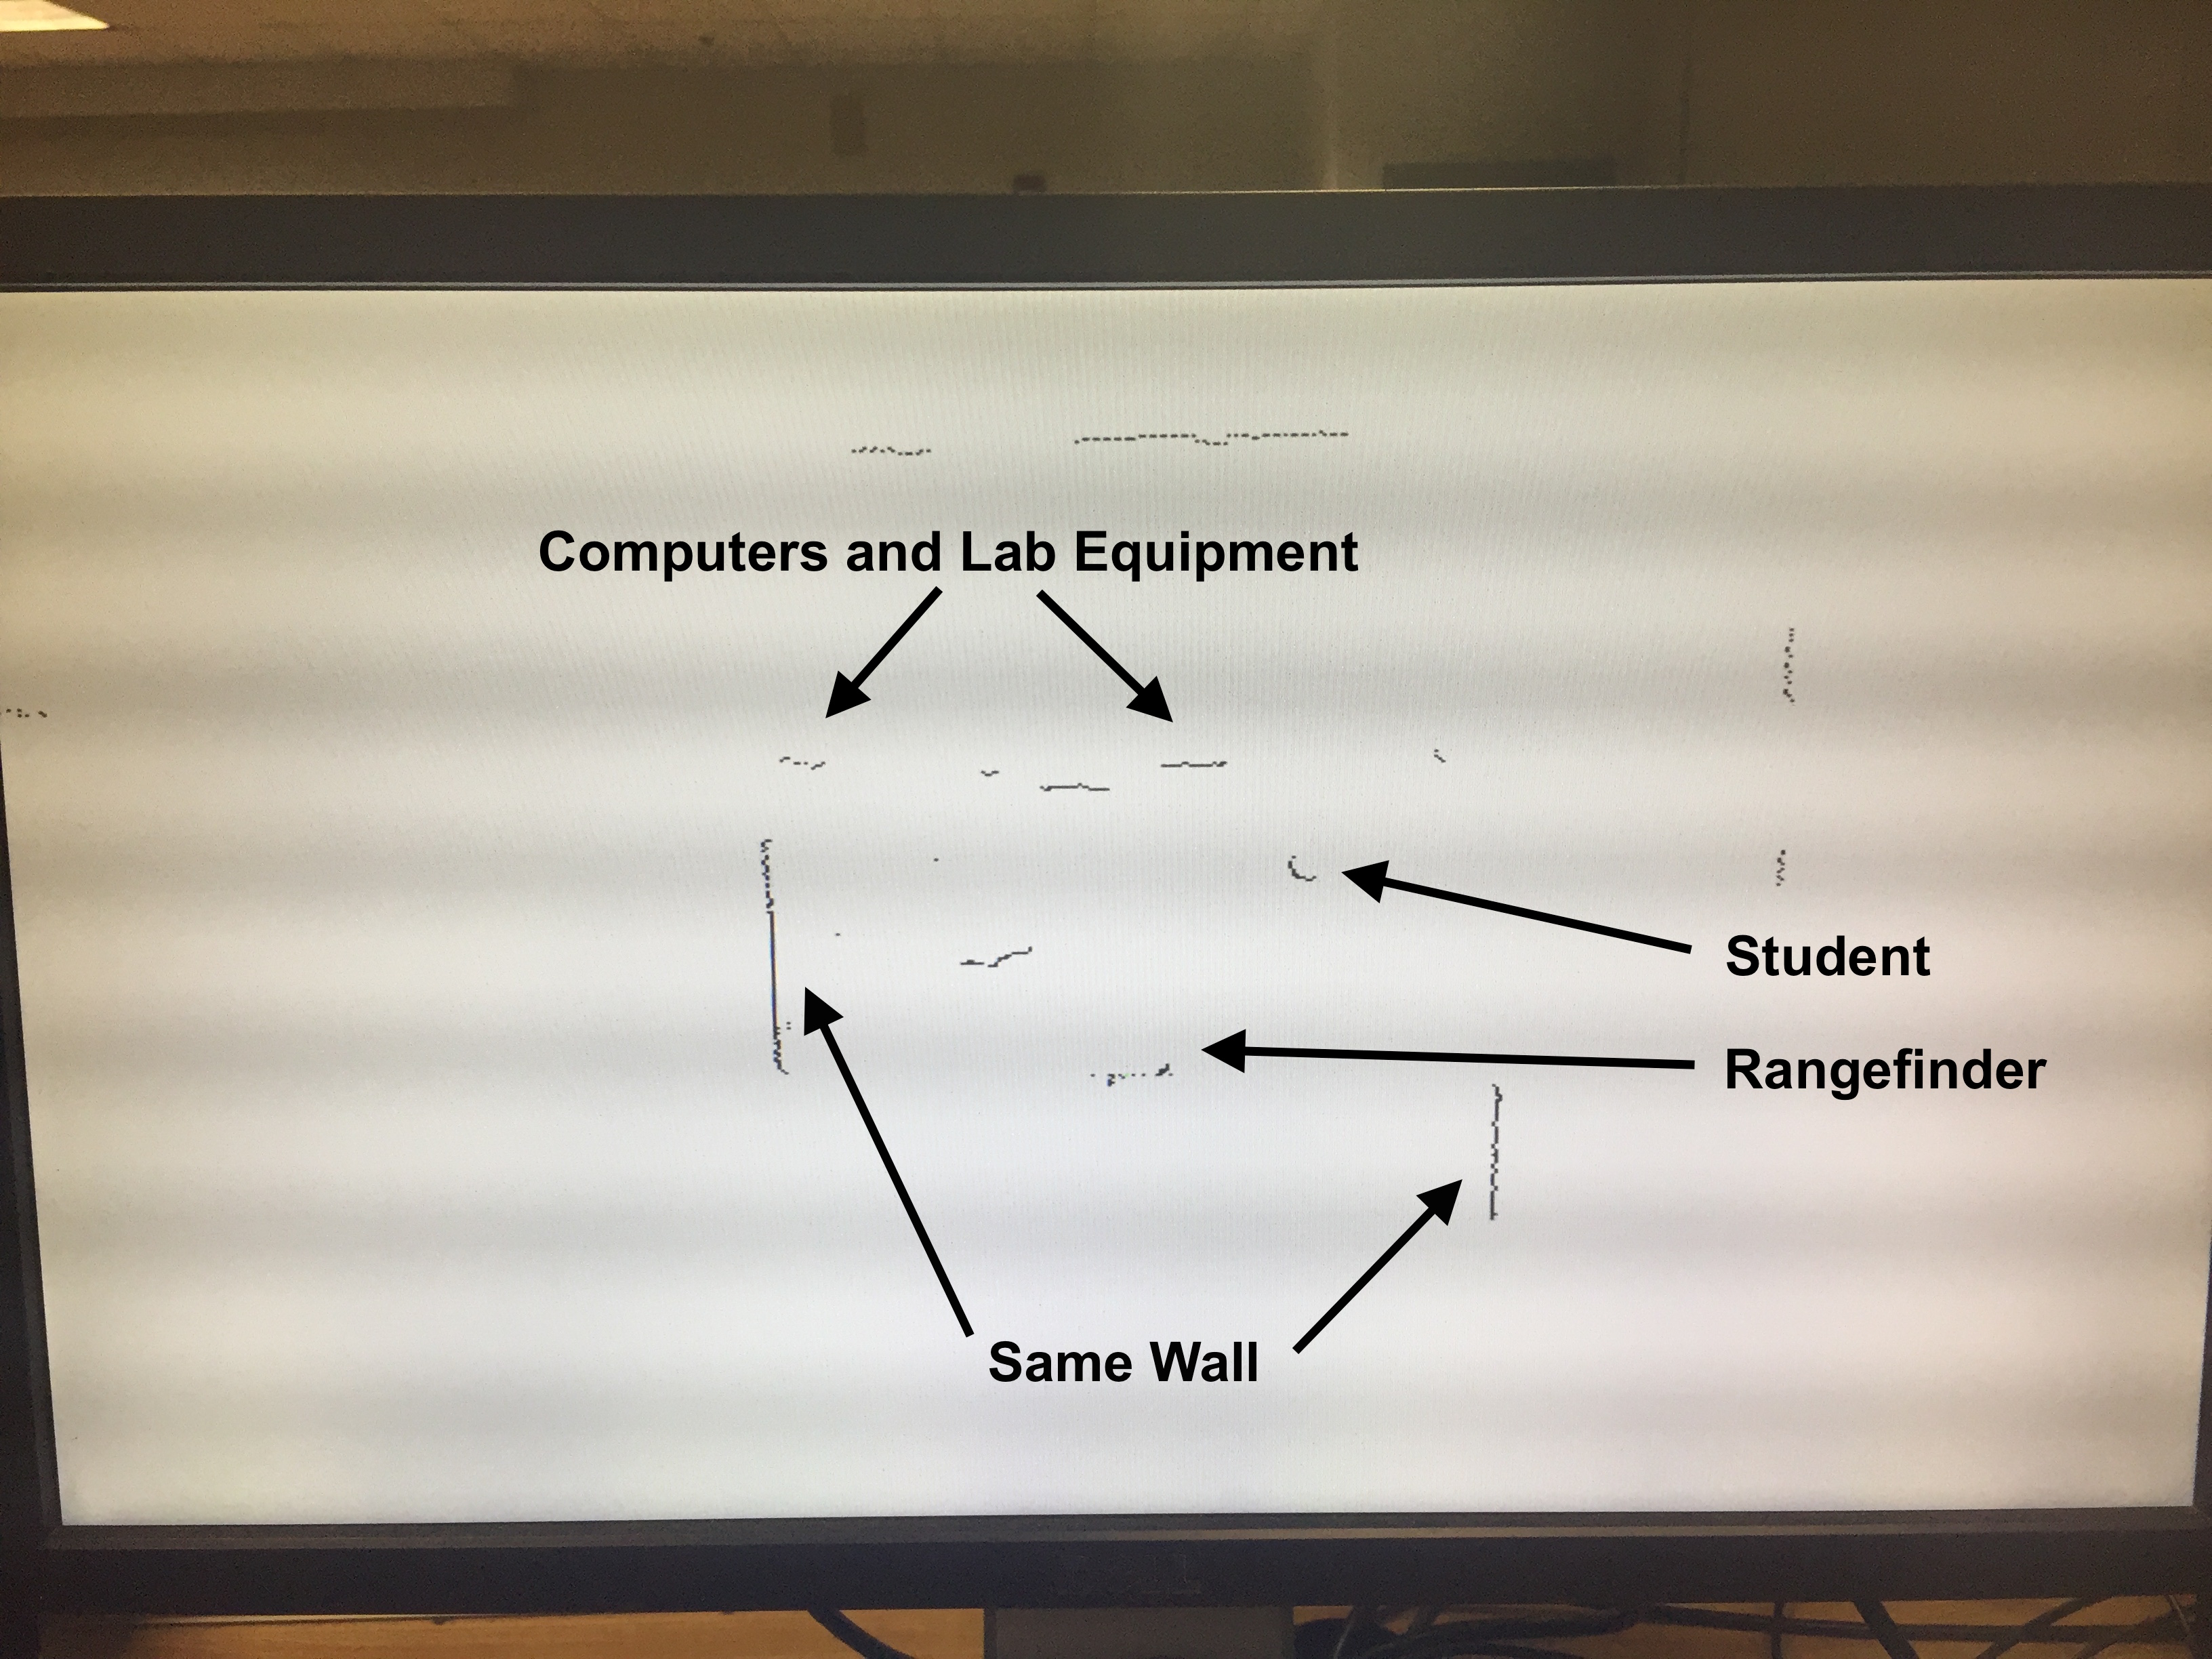
\includegraphics[width=0.8\linewidth]{lab_frontback.JPG}
		\caption{Two Overlaid Rangefinder "Floorplan" Captures with $180^\circ$ Offset}
		\label{resultant}
	\end{subfigure}
	\caption{Test of Rangefinder's Subsequent Triggering Functionality}
	\label{labtest2}
\end{figure}

This test confirmed that subsequent rangefinder data captures were triggered successfully and without loss of data. The floorplan shown in Figure \ref{labtest2}\subref{resultant} shows the data from the second trigger overlaid on top of the existing floorplan. The newly detected objects were called out in the figure. Note that although the rangefinder was rotated $180^\circ$, the floorplan did not account for that rotation. Because of this, it was possible for the same object to be detected in different places in subsequent data captures, as shown by the wall on each side of the rangefinder. This issue was resolved by incorporating the digital compass's rotational data in order to geographically reference the data. With the compass heading used to offset the direction of the device, 2D floorplan accurately reflected the relative location of objects.




